\begin{tikzpicture}
  \tikzset{et/.style={above,font=\footnotesize\vphantom{Ag}}}
  % 
  \node[inner sep=0pt, anchor=south west] (image) at (0,0){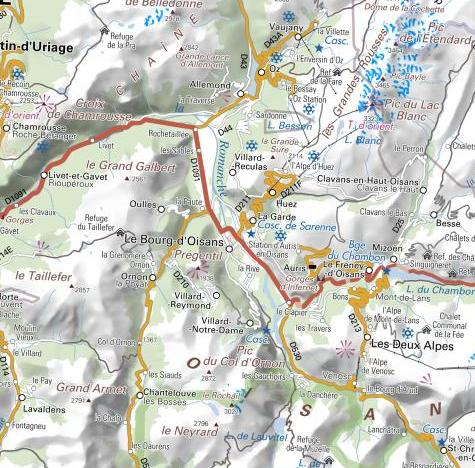
\includegraphics{./figures/bourdOisans.jpg}};
  % 
  \begin{scope}
    \node (P2) at ([yshift=-.5cm]image.south east) {};
    \node (P1) at ([yshift=-.5cm]image.south west) {};
    % Échelle
    \draw[-] (P2 |- -1cm,-1cm) --++ (-1,0) node[et,pos=.5] {\SI{2,500}{\kilo\meter}};
    % Légende détaillée
    \path (P1) -- (P2) node[pos=.5, yshift=-.2cm] {\tiny Source:
      Géoportail, SCAN régional IGN, 2020.};
  \end{scope}
\end{tikzpicture}